
\section{Tutorial}
\label{section:tutorial}
\setcounter{footnote}{0}

Here's a tutorial walk-through of how to use \rscape. This should
suffice to get you started.

\subsection {Modes of \rscape}

For an input alignment, \rscape\ reports all pairs that have
covariation scores with E-values smaller than a target E-value.\\

\noindent
R-scape has two different \textbf{modes} of operation which determine
how it calculates E-values, for which it needs to know how many
possible base pairs were tested (i.e. E-values are
multiple-test-corrected). The E-values are calculated in one of two ways:

\begin{tabular}{ll}
\multicolumn{2}{l}{\textbf{A one-set statistical test:} \textit{default}} \\ 
 & \\ 
\textbf{}   & E-values are calculated assuming that all pairs are possible.\\
\textbf{}   & This is the default behavior of \rscape.\\
 & \\ 
\multicolumn{2}{l}{\textbf{A two-set statistical test: } \prog{option -s}} \\ 
 & \\ 
\textbf{}   & If the alignment has associated a \emph{given structure}, \textbf{\prog{option -s}} performs two independent statistical tests: \\
\textbf{}   & one for the pairs included in the structure, a different one for all the remaining possible pairs.\\
\textbf{}   & It also draws the given consensus structure annotated with the significantly covarying base pairs.\\
 & \\ 
\end{tabular}

\subsection {The four options to run \rscape}

These are the four options to run R-scape.

\begin{labeling}{Evaluate region for conserved structure}
  
\item[Evaluate region for conserved structure]

  All possible pairs are analyzed equally as a one set test.  If a
  consensus structure is provided, that structure is ignored in the
  covariation test, but it is visualized with the significant
  covarying pairs highlighted in green.

  \textbf{preferred use:}\\
  This option is most appropriate if you're trying to determine if a conserved structure exists.\\
  
\item[Predict new structure]

  All possible pairs are analyzed equally.
  A structure is predicted and visualized with the significant covarying pairs highlighted in green.

  \textbf{preferred use:}\\
  This option is most appropriate for obtaining a new consensus
  structure prediction based on covariation analysis.

\item[Evaluate given structure]
  
  Requires that your Stockholm file has a proposed consensus structure annotation.
  Two independent covariation tests are performed, one on the set of proposed basepairs, the other on all other possible pairs.
  The given structure is visualized with significant covarying pairs highlighted in green.

  \textbf{preferred use:}\\
  This option is most appropriate for evaluating how well an
  independently proposed consensus structure is supported by
  covariation analysis.


\item[Improve given structure]

  Requires that your Stockholm file has a proposed consensus structure annotation.
  Two independent covariation tests are performed, one on the set of proposed basepairs, the other on all other possible pairs.
  A new consensus structure is predicted and visualized with the significant covarying pairs highlighted in green.

  \textbf{preferred use:}\\
  This option is most appropriate for using covariation analysis to improve your current consensus structure.

\end{labeling}



I'll show examples of running each mode, using examples in the
\ccode{tutorial/} subdirectory of the distribution.


\subsection {Option --RAF(S) disallowed}

The options to use the covariation measures RAF, RAFa, RAFp, RAFS, RAFSp, and RAFSa has
been disallowed, unless they are used in combination with option
--naive which reports the list of values for all possible pairs
without any statistical significance associated to them.

The following disclamer appears otherwise.

\user{bin/R-scape --RAF tutorial/updated\_Arisong.sto}\\

\begin{sreoutput}
DISCLAIMER: This measure can only be used in combination with the --naive option.

The --naive option reports a ranked list of scores for all possible
pairs without assigning E-values. RAF, RAFS and related measures
(RAFp, RAFa, RAFSp, RAFSa) cannot be used in combination with
R-scape's statistical test.

The RAF(S) statistics measure covariation and consistency. RAFS
assigns relatively high scores to pairs of alignment columns that are
consistent with base pairing even if there is no covariation at
all. The RAFS statistic was developed for the purpose of predicting
consensus RNA structures from alignments of sequences already presumed
to have a structure (Hofacker et al., 2002; Lindgreen et al.,
2006). For this purpose, both covariation and consistency are useful
cues. Distinguishing a conserved RNA structure from a conserved
primary sequence is a different problem that requires using a
statistic that does not systematically detect significant signals on
conserved primary sequence alone. That is R-scape's statistical
test. The R-scape statistical test can only be used with measures that
estimate covariation alone such as mutual information (MI) or G-test
(GT).
\end{sreoutput}

\subsection{Files used in the tutorial}

The subdirectory \prog{/tutorial} in the \rscape\ distribution contains the
files used in the tutorial. 

The tutorial provides several examples of RNA structural
alignments, all in Stockholm format:

\begin{sreitems}{\emprog{updated\_Arisong.sto}}
\item[\emprog{updated\_Arisong.sto}] Structural alignment of the ciliate
  Arisong RNA. This alignment is an updated
  version of the one published in~\citep{JungEddy11}.
\item[\emprog{ar14.sto}] Structural alignment of the $\alpha$-proteobacteria ncRNA ar14. This alignment is an updated version of the one
  published in~\citep{delVal12}.
\item[\emprog{manA.sto}] Alignment of the manA RNA motif~\citep{Weinberg09,Weinberg10} provided in the Zasha Weinberg database (ZWD)~\citep{ZWD18}.
\item[\emprog{RF00005.sto}] Rfam v12.0~\citep{Nawrocki15} seed alignment of tRNA. 
\item[\emprog{RF00001-noss.sto}] Rfam v12.0 seed alignment of 5S rRNA, after removing the consensus secondary structure. 
\end{sreitems}


\subsection{Running \rscape\, on one alignment file}
To run \rscape\ with default parameters on alignment file
\prog{tutorial/updated\_Arisong.sto} use:\\

\user{bin/R-scape tutorial/updated\_Arisong.sto}\\

\noindent
The output is a list of the significantly covarying positions under the one-set test

\begin{sreoutput}
# R-scape :: RNA Structural Covariation Above Phylogenetic Expectation
# R-scape 1.4.0 (Oct 2019)
# Copyright (C) 2016 Howard Hughes Medical Institute.
# Freely distributed under the GNU General Public License (GPLv3).
#-------------------------------------------------------------------------------------------------------
# MSA updated_Arisong_1 nseq 95 (95) alen 66 (150) avgid 65.82 (64.97) nbpairs 20 (20)
# One-set statistical test (all pairs are tested as equivalent) 
#
#
# Method Target_E-val [cov_min,cov_max] [FP | TP True Found | Sen PPV F] 
# GTp    0.05         [-9.78,121.66]     [0 | 2 20 2 | 10.00 100.00 18.18] 
#
#       left_pos       right_pos        score          E-value       substitutions      power
#-------------------------------------------------------------------------------------------------------
*	      98	     106	121.65645	0.00241628	45		0.48
*	     122	     137	91.44593	0.038356	57		0.58
\end{sreoutput}
A star ``*'' in the first column indicates that the pair is part of
the annotated structure in the \prog{updated\_Arisong.sto} file. A
blank indicates a pair that is not compatible with the structure. A
``$\sim$`` indicates an interaction not in the annotated structure but
compatible with it (none in this example).

The Arisong RNA in \prog{tutorial/updated\_Arisong.sto} has a proposed
secondary structure.  Instead of testing all pairs as equivalent, we
may want to test the significance of the given structure as a one set
of pairs, and independently that of the rest of all possible pairs.
In order to do a two-set test use:\\

\user{bin/R-scape -s tutorial/updated\_Arisong.sto}\\

\noindent
The output is a list of the significantly covarying positions under the two-set test.

\begin{sreoutput}
# R-scape :: RNA Structural Covariation Above Phylogenetic Expectation
# R-scape 1.4.0 (Oct 2019)
# Copyright (C) 2016 Howard Hughes Medical Institute.
# Freely distributed under the GNU General Public License (GPLv3).
#-------------------------------------------------------------------------------------------------------
# MSA updated_Arisong_1 nseq 95 (95) alen 66 (150) avgid 65.82 (64.97) nbpairs 20 (20)
# Two-set statistical test (one test for annotated basepairs, another for all other pairs)
#
#
# Method Target_E-val [cov_min,cov_max] [FP | TP True Found | Sen PPV F] 
# GTp    0.05         [-9.78,121.66]     [0 | 11 20 11 | 55.00 100.00 70.97] 
#
#       left_pos       right_pos        score          E-value       substitutions      power
#-------------------------------------------------------------------------------------------------------
*	      98	     106	121.65645	2.25295e-05	45		0.48
*	     122	     137	91.44593	0.000357632	57		0.58
*	      96	     108	88.43400	0.000466924	26		0.28
*	     120	     139	74.80289	0.00162024	87		0.76
*	     119	     140	58.72158	0.00678565	90		0.78
*	     121	     138	58.34837	0.00691674	99		0.82
*	      94	     110	57.27959	0.00760538	37		0.40
*	     124	     134	55.67692	0.0086606	20		0.21
*	     123	     135	54.59630	0.00946822	72		0.68
*	      99	     105	53.44797	0.0107226	15		0.14
*	      97	     107	44.91842	0.0405594	58		0.59

# The given structure
# SS_cons ::::::::::::::::::::::::::::::::::::::::::::::::::::::::::::
#
# SS_cons :::::::::::::::::::::::::::::::::<<<<<<<___>>>>>>><<<<<<--<<
#
# SS_cons <<<<<_______>>>->>>>-->>>>>>::
#

# Power analysis of given structure 
#
# covary  left_pos      right_pos    substitutions      power
#----------------------------------------------------------------
     *    94		110		37		0.40
          95		109		28		0.31
     *    96		108		26		0.28
     *    97		107		58		0.59
     *    98		106		45		0.48
     *    99		105		15		0.14
          100		104		20		0.21
          111		148		0		0.00
          112		147		18		0.18
          113		146		1		0.00
          114		145		15		0.14
          115		144		49		0.52
          116		143		106		0.84
     *    119		140		90		0.78
     *    120		139		87		0.76
     *    121		138		99		0.82
     *    122		137		57		0.58
     *    123		135		72		0.68
     *    124		134		20		0.21
          125		133		31		0.34
#
# BPAIRS 20
# avg substitutions per BP  43.7
# BPAIRS expected to covary 8.3
# BPAIRS observed to covary 11
\end{sreoutput}
The scores of the pairs are identical to those in the one-set
test. The E-values have changed relative to those of the one-set test.


\subsection{The --fold option}

After performing one of the two statistical tests, this option implements the CaCoFold algorithm:\\

\begin{tabular}{ll}
\textbf{}   & Builds the best consensus structure that includes the largest possible number of significantly covarying pairs,\\
\textbf{}   & \hspace{5mm}\emph{the maximum-covariation optimal consensus structure}. The algorithm identifies pseudoknots and\\
\textbf{}   & \hspace{5mm}other not nested interactions by running a cascade of nested algorithms until all covarying pairs\\
\textbf{}   & \hspace{5mm}are taken into account.\\
\textbf{}   & Draws the \emph{maximum-covariation optimal consensus structure} annotated with the significantly \\
\textbf{}   & \hspace{5mm}covarying base pairs.\\
\textbf{}   & It also returns the alignment in Stockholm format annotated with the max-cov optimal consensus structure.\\
 & \\ 
\end{tabular}

\user{bin/R-scape --fold tutorial/updated\_Arisong.sto}\\

\noindent
The output includes first the same output as default \rscape\ alone,
followed by \rscape's proposed structure that under the heading ``\#
The predicted CaCoFold structure'' as follows,

\begin{sreoutput}
# The predicted CaCoFold structure
# SS_cons ::::::::::::::::::::::::::::::::::::::::::::::::::::::::::::
#
# SS_cons ::::::::::::::::::::::::::::::::::<<<<<_____>>>>>:<<<<<---<<
#
# SS_cons <<<<_________>>->>>>--->>>>>::
#

# Power analysis of CaCoFold structure 
#
# covary  left_pos      right_pos    substitutions      power
#----------------------------------------------------------------
          95		109		28		0.31
          96		108		26		0.28
          97		107		58		0.59
     *    98		106		45		0.48
          99		105		15		0.14
          111		148		0		0.00
          112		147		18		0.18
          113		146		1		0.00
          114		145		15		0.14
          115		144		49		0.52
          119		140		90		0.78
          120		139		87		0.76
          121		138		99		0.82
     *    122		137		57		0.58
          123		135		72		0.68
          124		134		20		0.21
#
# BPAIRS 16
# avg substitutions per BP  42.5
# BPAIRS expected to covary 6.5
# BPAIRS observed to covary 2
\end{sreoutput}

The structure predicted by \rscape\ includes all the basepairs
reported as covarying, provided that those can be arranged into one
single structure (including pseudoknots and other non Watson-Crick
interactions). The \rscape\ folding algorithm cannot deal with
residues that covary with more than one other residue, such as is the case for
alternative structures or triplets.

\noindent
Similarly using

\user{bin/R-scape -s --fold tutorial/updated\_Arisong.sto}\\

\noindent
The output includes first the same output as \emprog{option -s} of
\rscape\ alone, followed by \rscape's proposed CaCoFild structure including all the 
the covarying pairs  obtained under the two-set test.

\begin{sreoutput}
# R-scape :: RNA Structural Covariation Above Phylogenetic Expectation
# R-scape 1.4.0 (Oct 2019)
# Copyright (C) 2016 Howard Hughes Medical Institute.
# Freely distributed under the GNU General Public License (GPLv3).
#-------------------------------------------------------------------------------------------------------
# MSA updated_Arisong_1 nseq 95 (95) alen 66 (150) avgid 65.82 (64.97) nbpairs 20 (20)
# Two-set statistical test (one test for annotated basepairs, another for all other pairs)
#
#
# Method Target_E-val [cov_min,cov_max] [FP | TP True Found | Sen PPV F] 
# GTp    0.05         [-9.78,121.66]     [0 | 11 20 11 | 55.00 100.00 70.97] 
#
#       left_pos       right_pos        score          E-value       substitutions      power
#-------------------------------------------------------------------------------------------------------
*	      98	     106	121.65645	2.25295e-05	45		0.48
*	     122	     137	91.44593	0.000357632	57		0.58
*	      96	     108	88.43400	0.000466924	26		0.28
*	     120	     139	74.80289	0.00162024	87		0.76
*	     119	     140	58.72158	0.00678565	90		0.78
*	     121	     138	58.34837	0.00691674	99		0.82
*	      94	     110	57.27959	0.00760538	37		0.40
*	     124	     134	55.67692	0.0086606	20		0.21
*	     123	     135	54.59630	0.00946822	72		0.68
*	      99	     105	53.44797	0.0107226	15		0.14
*	      97	     107	44.91842	0.0405594	58		0.59

# The given structure
# SS_cons ::::::::::::::::::::::::::::::::::::::::::::::::::::::::::::
#
# SS_cons :::::::::::::::::::::::::::::::::<<<<<<<___>>>>>>><<<<<<--<<
#
# SS_cons <<<<<_______>>>->>>>-->>>>>>::
#

# Power analysis of given structure 
#
# covary  left_pos      right_pos    substitutions      power
#----------------------------------------------------------------
     *    94		110		37		0.40
          95		109		28		0.31
     *    96		108		26		0.28
     *    97		107		58		0.59
     *    98		106		45		0.48
     *    99		105		15		0.14
          100		104		20		0.21
          111		148		0		0.00
          112		147		18		0.18
          113		146		1		0.00
          114		145		15		0.14
          115		144		49		0.52
          116		143		106		0.84
     *    119		140		90		0.78
     *    120		139		87		0.76
     *    121		138		99		0.82
     *    122		137		57		0.58
     *    123		135		72		0.68
     *    124		134		20		0.21
          125		133		31		0.34
#
# BPAIRS 20
# avg substitutions per BP  43.7
# BPAIRS expected to covary 8.3
# BPAIRS observed to covary 11
#
#
# Method Target_E-val [cov_min,cov_max] [FP | TP True Found | Sen PPV F] 
# GTp    0.05         [-9.78,121.66]     [0 | 11 17 11 | 64.71 100.00 78.57] 
#
# in_fold in_given   left_pos       right_pos      score           E-value    substitutions      power
#----------------------------------------------------------------------------------------------------------------
*	*	        98	       106	121.65645	2.25295e-05	45		0.48
*	*	       122	       137	91.44593	0.000357632	57		0.58
*	*	        96	       108	88.43400	0.000466924	26		0.28
*	*	       120	       139	74.80289	0.00162024	87		0.76
*	*	       119	       140	58.72158	0.00678565	90		0.78
*	*	       121	       138	58.34837	0.00691674	99		0.82
*	*	        94	       110	57.27959	0.00760538	37		0.40
*	*	       124	       134	55.67692	0.0086606	20		0.21
*	*	       123	       135	54.59630	0.00946822	72		0.68
*	*	        99	       105	53.44797	0.0107226	15		0.14
*	*	        97	       107	44.91842	0.0405594	58		0.59

# The predicted CaCoFold structure
# SS_cons ::::::::::::::::::::::::::::::::::::::::::::::::::::::::::::
#
# SS_cons :::::::::::::::::::::::::::::::::<<<<<<_____>>>>>><<<<<---<<
#
# SS_cons <<<<_________>>->>>>--->>>>>::
#

# Power analysis of CaCoFold structure 
#
# covary  left_pos      right_pos    substitutions      power
#----------------------------------------------------------------
     *    94		110		37		0.40
          95		109		28		0.31
     *    96		108		26		0.28
     *    97		107		58		0.59
     *    98		106		45		0.48
     *    99		105		15		0.14
          111		148		0		0.00
          112		147		18		0.18
          113		146		1		0.00
          114		145		15		0.14
          115		144		49		0.52
     *    119		140		90		0.78
     *    120		139		87		0.76
     *    121		138		99		0.82
     *    122		137		57		0.58
     *    123		135		72		0.68
     *    124		134		20		0.21
#
# BPAIRS 17
# avg substitutions per BP  42.2
# BPAIRS expected to covary 6.9
# BPAIRS observed to covary 11
\end{sreoutput}


\subsection{Example of an RNA with pseudoknots}

\rscape\ implements the CaCoFold folding algorithm capable of
predicting pseudoknots and other non nested interactions using a
cascade of dynamic programming algorithms.  \rscape\ had adapted the
program R2R to automatically include in the display all covarying
interactions whether they are nested or not.

Consider the manA RNA motif. Both the proposed structure for manA RNA
and the predicted CaCoFold structure have 2 pseudoknots with
covariation support:

\user{bin/R-scape -s --fold tutorial/manA.sto}\\

\begin{sreoutput}
# The given structure
# SS_cons   <<<<<<_______________________________>>>>>>:::::[[[[[,,,<<--
# SS_cons_1 ::::::::::::::::::::::::::::::::::::::::::::::::::::::::::::
# SS_cons_2 ::::::::::::::::::::::::::::::::::::::::::::::::::::::::::::
#
# SS_cons   -----------<<<<<<__________________>>>>>>---->>,,,,((-((((,,
# SS_cons_1 ::::::::::::::::::::::::::::::::::::::::::::::::::::::::::::
# SS_cons_2 ::::::::::::::::::::::::::::::::::::::::::::::::::::::::::::
#
# SS_cons   ,,,,,,,,,,,,,,,,,,,,,,,,,,,,,<<<_______>>>,<<<<<<___________
# SS_cons_1 ::::::::::::::::::::::::::::::::::<<<<______________________
# SS_cons_2 ::::::::::::::::::::::::::::::::::::::::::::::::::::::::::::
#
# SS_cons   ____________________>>>>>>,,,<<<<<____________>>>>>,,))))--)
# SS_cons_1 _______________________________________>>>>:::::::::::::::::
# SS_cons_2 ::::::::::::::::::::::::::::::::::::::::::::::::::::::::::::
#
# SS_cons   ),,,,<<<<<<<------------<<<<____________________________>>>>
# SS_cons_1 ::::::::::::::::::::::::::::::::::::::::::::::::::::::::::::
# SS_cons_2 :::::::::::::::::::::::::::::::::<<<-<______________________
#
# SS_cons   ------->>>>>>>,,<<<<<_____________>>>>>]]]]]::::::
# SS_cons_1 ::::::::::::::::::::::::::::::::::::::::::::::::::
# SS_cons_2 _________________________>>>>:::::::::::::::::::::
#

# Power analysis of given structure 
#
# covary  left_pos      right_pos    substitutions      power
#----------------------------------------------------------------
     *    1		43		61		0.61
     *    2		42		61		0.61
     *    3		41		72		0.68
     *    4		40		104		0.83
     *    5		39		106		0.84
     *    6		38		126		0.90
          49		344		15		0.14
     *    50		343		16		0.16
     *    51		342		26		0.28
     *    52		341		77		0.71
     *    53		340		26		0.28
     *    57		107		38		0.41
     *    58		106		16		0.16
     *    72		101		71		0.68
     *    73		100		38		0.41
     *    74		99		60		0.60
     *    75		98		34		0.37
     *    76		97		31		0.34
          77		96		27		0.30
     *    112		241		41		0.44
     *    113		240		51		0.53
     *    115		237		61		0.61
     *    116		236		46		0.49
     *    117		235		62		0.62
     *    118		234		49		0.52
     *    150		162		52		0.54
     *    151		161		47		0.50
     *    152		160		36		0.39
          155		223		31		0.34
     *    156		222		30		0.33
          157		221		28		0.31
          158		220		27		0.30
     *    164		206		29		0.32
     *    165		205		54		0.56
     *    166		204		148		0.94
     *    167		203		109		0.85
     *    168		202		154		0.95
     *    169		201		147		0.94
          210		231		48		0.51
     *    211		230		77		0.71
     *    212		229		71		0.68
     *    213		228		59		0.60
     *    214		227		75		0.70
     *    246		314		62		0.62
     *    247		313		92		0.79
     *    248		312		141		0.93
     *    249		311		90		0.78
     *    250		310		99		0.82
     *    251		309		105		0.84
     *    252		308		37		0.40
     *    265		300		61		0.61
     *    266		299		44		0.47
     *    267		298		42		0.45
     *    268		297		36		0.39
     *    274		329		47		0.50
     *    275		328		36		0.39
     *    276		327		39		0.42
          278		326		42		0.45
          317		339		13		0.12
     *    318		338		37		0.40
     *    319		337		60		0.60
     *    320		336		18		0.18
          321		335		0		0.00
#
# BPAIRS 63
# avg substitutions per BP  57.7
# BPAIRS expected to covary 33.2
# BPAIRS observed to covary 54

  ...

  ...
  
# The predicted CaCoFold structure
# SS_cons   <<<<<<_______________________________>>>>>>:[---[[[[[,,,<<--
# SS_cons_1 ::::::::::::::::::::::::::::::::::::::::::::::::::::::::::::
# SS_cons_2 ::::::::::::::::::::::::::::::::::::::::::::::::::::::::::::
#
# SS_cons   -----------<<<<<<__________________>>>>>>---->>,(--((-((((,,
# SS_cons_1 ::::::::::::::::::::::::::::::::::::::::::::::::::::::::::::
# SS_cons_2 ::::::::::::::::::::::::::::::::::::::::::::::::::::::::::::
#
# SS_cons   ,,,,,,,,,,,,,,,,,,,,,,,,,,,,,<<<_______>>>,<<<<<<___________
# SS_cons_1 ::::::::::::::::::::::::::::::::::<<<<______________________
# SS_cons_2 ::::::::::::::::::::::::::::::::::::::::::::::::::::::::::::
#
# SS_cons   ____________________>>>>>>,,,<<<<<---<____>--->>>>>,,))))--)
# SS_cons_1 _______________________________________>>>>:::::::::::::::::
# SS_cons_2 ::::::::::::::::::::::::::::::::::::::::::::::::::::::::::::
#
# SS_cons   )--),<<<<<<<------------<<<<-<<______>>----------------->>>>
# SS_cons_1 ::::::::::::::::::::::::::::::::::::::::::::::::::::::::::::
# SS_cons_2 :::::::::::::::::::::::::::::::::<<<-<______________________
#
# SS_cons   ------->>>>>>>,,<<<<<_____________>>>>>]]]]]-]::::
# SS_cons_1 ::::::::::::::::::::::::::::::::::::::::::::::::::
# SS_cons_2 _________________________>>>>:::::::::::::::::::::
#

# Power analysis of CaCoFold structure 
#
# covary  left_pos      right_pos    substitutions      power
#----------------------------------------------------------------
     *    1		43		61		0.61
     *    2		42		61		0.61
     *    3		41		72		0.68
     *    4		40		104		0.83
     *    5		39		106		0.84
     *    6		38		126		0.90
          45		346		82		0.74
          49		344		15		0.14
     *    50		343		16		0.16
     *    51		342		26		0.28
     *    52		341		77		0.71
     *    53		340		26		0.28
     *    57		107		38		0.41
     *    58		106		16		0.16
     *    72		101		71		0.68
     *    73		100		38		0.41
     *    74		99		60		0.60
     *    75		98		34		0.37
     *    76		97		31		0.34
          77		96		27		0.30
     *    109		244		37		0.40
     *    112		241		41		0.44
     *    113		240		51		0.53
     *    115		237		61		0.61
     *    116		236		46		0.49
     *    117		235		62		0.62
     *    118		234		49		0.52
     *    150		162		52		0.54
     *    151		161		47		0.50
     *    152		160		36		0.39
          155		223		31		0.34
     *    156		222		30		0.33
          157		221		28		0.31
          158		220		27		0.30
     *    164		206		29		0.32
     *    165		205		54		0.56
     *    166		204		148		0.94
     *    167		203		109		0.85
     *    168		202		154		0.95
     *    169		201		147		0.94
          210		231		48		0.51
     *    211		230		77		0.71
     *    212		229		71		0.68
     *    213		228		59		0.60
     *    214		227		75		0.70
          218		223		59		0.60
     *    246		314		62		0.62
     *    247		313		92		0.79
     *    248		312		141		0.93
     *    249		311		90		0.78
     *    250		310		99		0.82
     *    251		309		105		0.84
     *    252		308		37		0.40
     *    265		300		61		0.61
     *    266		299		44		0.47
     *    267		298		42		0.45
     *    268		297		36		0.39
          270		279		47		0.50
          271		278		81		0.73
     *    274		329		47		0.50
     *    275		328		36		0.39
     *    276		327		39		0.42
          278		326		42		0.45
          317		339		13		0.12
     *    318		338		37		0.40
     *    319		337		60		0.60
     *    320		336		18		0.18
          321		335		0		0.00
#
# BPAIRS 68
# avg substitutions per BP  58.0
# BPAIRS expected to covary 36.2
# BPAIRS observed to covary 55
\end{sreoutput}

\noindent
 The ``SS\_cons\_1'' and ``SS\_cons\_2'' lines describe the
 interactions that are not nested relative to the main ``SS\_cons''
 structure.

\rscape\, uses R2R to produce figures of the consensus structures
where pseudoknots are also annotated.  \rscape] option -s produces the
  file \emprog{tutorial/manA.R2R.sto.\{pdf,svg\}} with the structure
  annotated in the input alignment. \rscape] option --fold produces the
    file \emprog{tutorial/manA.fold.R2R.sto.\{pdf,svg\}} with the
    structure produced by \rscape. See Figure~\ref{fig:manA_r2r}.


 \begin{figure}[h]
   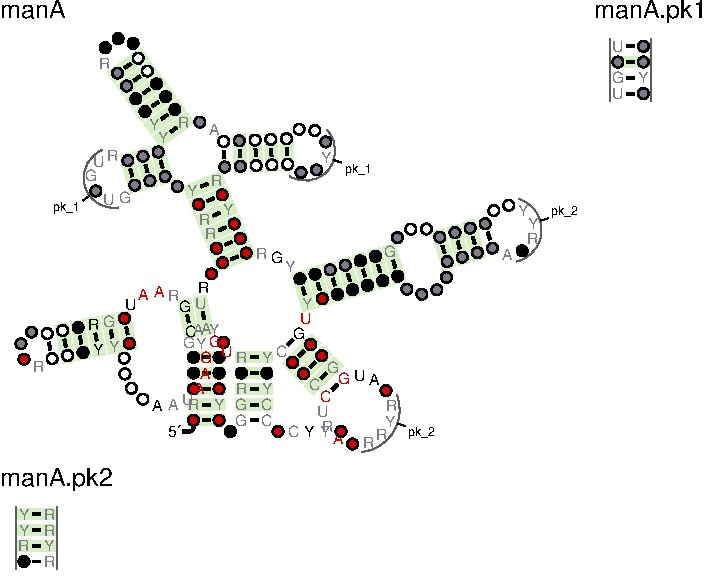
\includegraphics[scale=0.7]{manA_R2R.pdf} 
  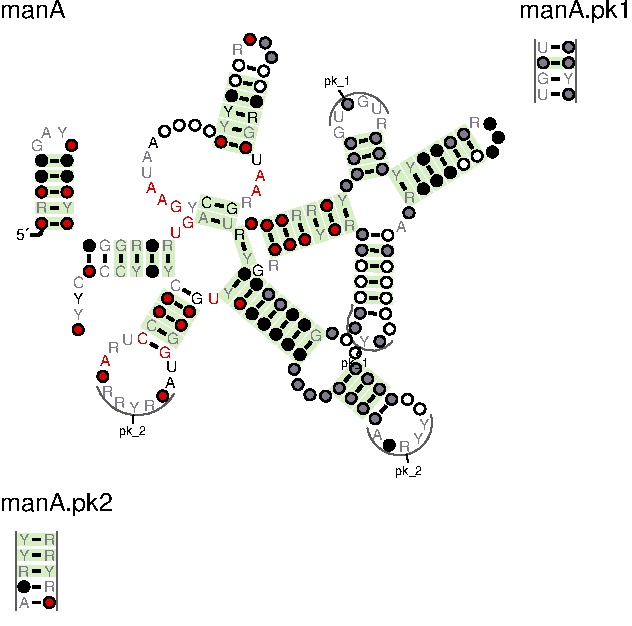
\includegraphics[scale=0.7]{manA_fold_R2R.pdf} 
  \caption{\small\textbf{Left:}
    \emprog{tutorial/manA.R2R.sto.\{pdf,svg\}}, the consensus
    secondary structure given in the input alignment, depicted by
    \rscape, using the program R2R.  \textbf{Right:}
    \emprog{tutorial/manA.fold.R2R.sto.\{pdf,svg\}}, The consensus
    structure produced by \rscape\ (option --fold).  Base pairs with
    covariation scores equal or below the target E-value (0.05 as
    default) are depicted in green.  }
 \label{fig:manA_r2r}
 \end{figure}
 

 \subsection{Single sequence structure prediction}

 If the alignment includes only one sequence, no statistical test is performed. \\

 \noindent
 \user{bin/R-scape --fold tutorial/manA-oneseq.sto}\\
%
 reports the best structure given the sequence. No covariation support
 is possible for any of the basepairs reported from this
 analysis. Structures produced this way have to taken with great
 skepticism. 

 \subsection{Default parameters}

Default parameters are:

\begin{sreitems}{\emprog{Pairwise percent identity:}}
\item[\emprog{Target E-value:}]default is 0.05. \rscape\, reports
  pairs which covariation score has E-value smaller or equal to the
  target value.  The target E-value can be changed with option
  \emprog{-E <x>}, $x >= 0$.

\item[\emprog{Sequence weighting:}]Sequences are weighted according to
  the Gerstein/Sonnhammer/Chothia (GSC)
  algorithm~\citep{Gerstein94}. This algorithm is time consuming. For
  alignments with more than 1000 sequences, we use the faster
  position-based weighting algorithm~\citep{Henikoff94b}. Both
  weighting algorithms are implemented as part of the easel library.

\item[\emprog{Gaps in columns:}]Columns with more than 50\% gaps are
  removed. The gap threshold for removing columns can be modified
   using option \emprog{--gapthresh <x>} , $0<x<=1$.

 \item[\emprog{Covariation statistic:}]The default covariation statistic
   is the average product corrected G-Test (equivalent to option
   \emprog{--GTp}).

 \item[\emprog{Covariation Class:}]\rscape\ uses the 16 component
   covariation statistic (C16), unless the number of sequences in the
   alignment is $\leq$ 8 or the length of the alignment is $\leq$ 50,
   in which case it uses the two-class covariation statistic (C2). A
   particular covariation class can be selected using either
   \emprog{--C16} or \emprog{--C2}.

   The threshold for the minimum number of sequences can be changed
   with option \prog{--nseqthresh <n>}.  The threshold for the minimum
   alignment length can be changed with option \prog{--alenthresh <n>}.

 \item[\emprog{Null alignments:}]In order to estimate E-values,
   \rscape\ produces 20 null alignments, unless the product of the
   number of sequences by the length of the alignment $<$ 10,000 in
   which case the number of null alignments is 50; or $<$ 1,000 in
   which case it is 100. The number of null alignments can be
   controlled with option \emprog{--nshuffle <n>}.
 \end{sreitems}

 A full list of the \rscape\ options is found by using

 \user{\rscape\ -h}

 
 
